\PassOptionsToPackage{unicode=true}{hyperref} % options for packages loaded elsewhere
\PassOptionsToPackage{hyphens}{url}
%
\documentclass[
  ignorenonframetext,
]{beamer}
\usepackage{pgfpages}
\setbeamertemplate{caption}[numbered]
\setbeamertemplate{caption label separator}{: }
\setbeamercolor{caption name}{fg=normal text.fg}
\beamertemplatenavigationsymbolsempty
% Prevent slide breaks in the middle of a paragraph:
\widowpenalties 1 10000
\raggedbottom
\setbeamertemplate{part page}{
  \centering
  \begin{beamercolorbox}[sep=16pt,center]{part title}
    \usebeamerfont{part title}\insertpart\par
  \end{beamercolorbox}
}
\setbeamertemplate{section page}{
  \centering
  \begin{beamercolorbox}[sep=12pt,center]{part title}
    \usebeamerfont{section title}\insertsection\par
  \end{beamercolorbox}
}
\setbeamertemplate{subsection page}{
  \centering
  \begin{beamercolorbox}[sep=8pt,center]{part title}
    \usebeamerfont{subsection title}\insertsubsection\par
  \end{beamercolorbox}
}
\AtBeginPart{
  \frame{\partpage}
}
\AtBeginSection{
  \ifbibliography
  \else
    \frame{\sectionpage}
  \fi
}
\AtBeginSubsection{
  \frame{\subsectionpage}
}
\usepackage{lmodern}
\usepackage{amssymb,amsmath}
\usepackage{ifxetex,ifluatex}
\ifnum 0\ifxetex 1\fi\ifluatex 1\fi=0 % if pdftex
  \usepackage[T1]{fontenc}
  \usepackage[utf8]{inputenc}
  \usepackage{textcomp} % provides euro and other symbols
\else % if luatex or xelatex
  \usepackage{unicode-math}
  \defaultfontfeatures{Scale=MatchLowercase}
  \defaultfontfeatures[\rmfamily]{Ligatures=TeX,Scale=1}
\fi
\usetheme[]{CambridgeUS}
\usecolortheme{dove}
\usefonttheme{professionalfonts}
% use upquote if available, for straight quotes in verbatim environments
\IfFileExists{upquote.sty}{\usepackage{upquote}}{}
\IfFileExists{microtype.sty}{% use microtype if available
  \usepackage[]{microtype}
  \UseMicrotypeSet[protrusion]{basicmath} % disable protrusion for tt fonts
}{}
\makeatletter
\@ifundefined{KOMAClassName}{% if non-KOMA class
  \IfFileExists{parskip.sty}{%
    \usepackage{parskip}
  }{% else
    \setlength{\parindent}{0pt}
    \setlength{\parskip}{6pt plus 2pt minus 1pt}}
}{% if KOMA class
  \KOMAoptions{parskip=half}}
\makeatother
\usepackage{xcolor}
\IfFileExists{xurl.sty}{\usepackage{xurl}}{} % add URL line breaks if available
\IfFileExists{bookmark.sty}{\usepackage{bookmark}}{\usepackage{hyperref}}
\hypersetup{
  pdftitle={Allele},
  pdfauthor={JK},
  pdfborder={0 0 0},
  breaklinks=true}
\urlstyle{same}  % don't use monospace font for urls
\newif\ifbibliography
\usepackage{graphicx,grffile}
\makeatletter
\def\maxwidth{\ifdim\Gin@nat@width>\linewidth\linewidth\else\Gin@nat@width\fi}
\def\maxheight{\ifdim\Gin@nat@height>\textheight\textheight\else\Gin@nat@height\fi}
\makeatother
% Scale images if necessary, so that they will not overflow the page
% margins by default, and it is still possible to overwrite the defaults
% using explicit options in \includegraphics[width, height, ...]{}
\setkeys{Gin}{width=\maxwidth,height=\maxheight,keepaspectratio}
\setlength{\emergencystretch}{3em}  % prevent overfull lines
\providecommand{\tightlist}{%
  \setlength{\itemsep}{0pt}\setlength{\parskip}{0pt}}
\setcounter{secnumdepth}{-2}

% set default figure placement to htbp
\makeatletter
\def\fps@figure{htbp}
\makeatother


\title{Allele}
\author{JK}
\date{2019 9 27}

\begin{document}
\frame{\titlepage}

\begin{frame}{BRCA result}
\protect\hypertarget{brca-result}{}

\begin{itemize}
\tightlist
\item
  BRCA1 mutation: Positive - p.Glu649Ter (c.1945G\textgreater{}T)\\
\item
  Variant allele frequency 63.84\%\\
\item
  Tumor cell percentage: 70\%\\
\item
  BRCA negative in blood sample
\end{itemize}

\end{frame}

\begin{frame}{Question}
\protect\hypertarget{question}{}

\begin{quote}
Is it possible \textbf{64\% allele frequency} of somatic mutation?
\end{quote}

\end{frame}

\begin{frame}{Variant allele frequency in clinical tumor sample}
\protect\hypertarget{variant-allele-frequency-in-clinical-tumor-sample}{}

\[Allele \space frequency \approx Read \space count\]
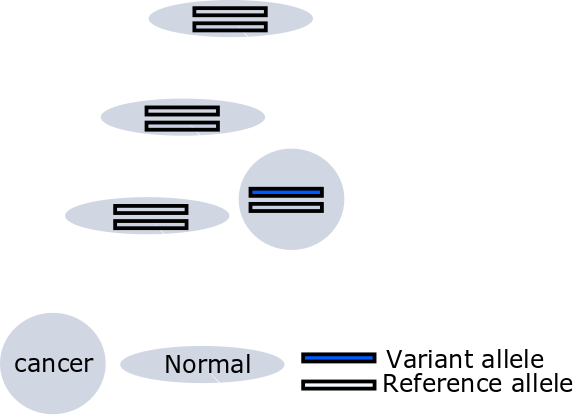
\includegraphics{img/Allele_3.png}

\end{frame}

\begin{frame}{Variant allele frequency in clinical tumor sample}
\protect\hypertarget{variant-allele-frequency-in-clinical-tumor-sample-1}{}

\begin{itemize}
\tightlist
\item
  Germline vs somatic\\
\item
  Tumor cell proportion\\
\item
  Copy number\\
\item
  Loss of heterozygosity
\end{itemize}

\end{frame}

\begin{frame}{Germline variant, Two copy, Heterozigosity, Tumor
cellularity 25\%}
\protect\hypertarget{germline-variant-two-copy-heterozigosity-tumor-cellularity-25}{}

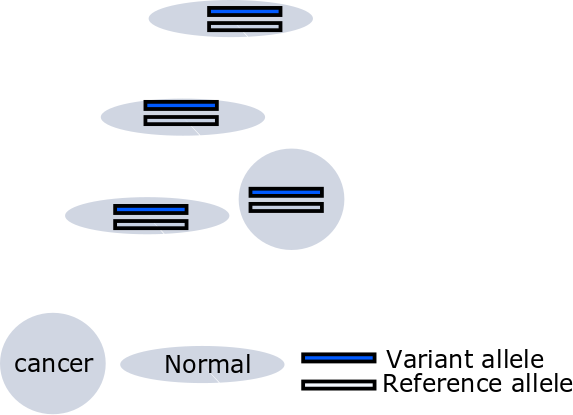
\includegraphics{img/Allele_2.png}\\
Variant allele frequency?

\end{frame}

\begin{frame}{Germline variant, One copy, LOH, Tumor cellularity 100\%}
\protect\hypertarget{germline-variant-one-copy-loh-tumor-cellularity-100}{}

\begin{quote}
Allele frequency 100\% \textbf{hetero germline} variant
\end{quote}

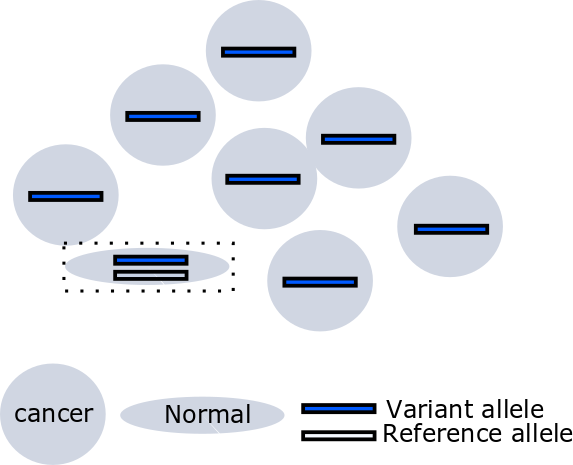
\includegraphics{img/Allele_7.png}

\end{frame}

\begin{frame}{Allele frequency in Somatic vs Germline in tumor only
sample\textsuperscript{1}}
\protect\hypertarget{allele-frequency-in-somatic-vs-germline-in-tumor-only-sample-sun_2018_computational_ploscomputationalbiology}{}

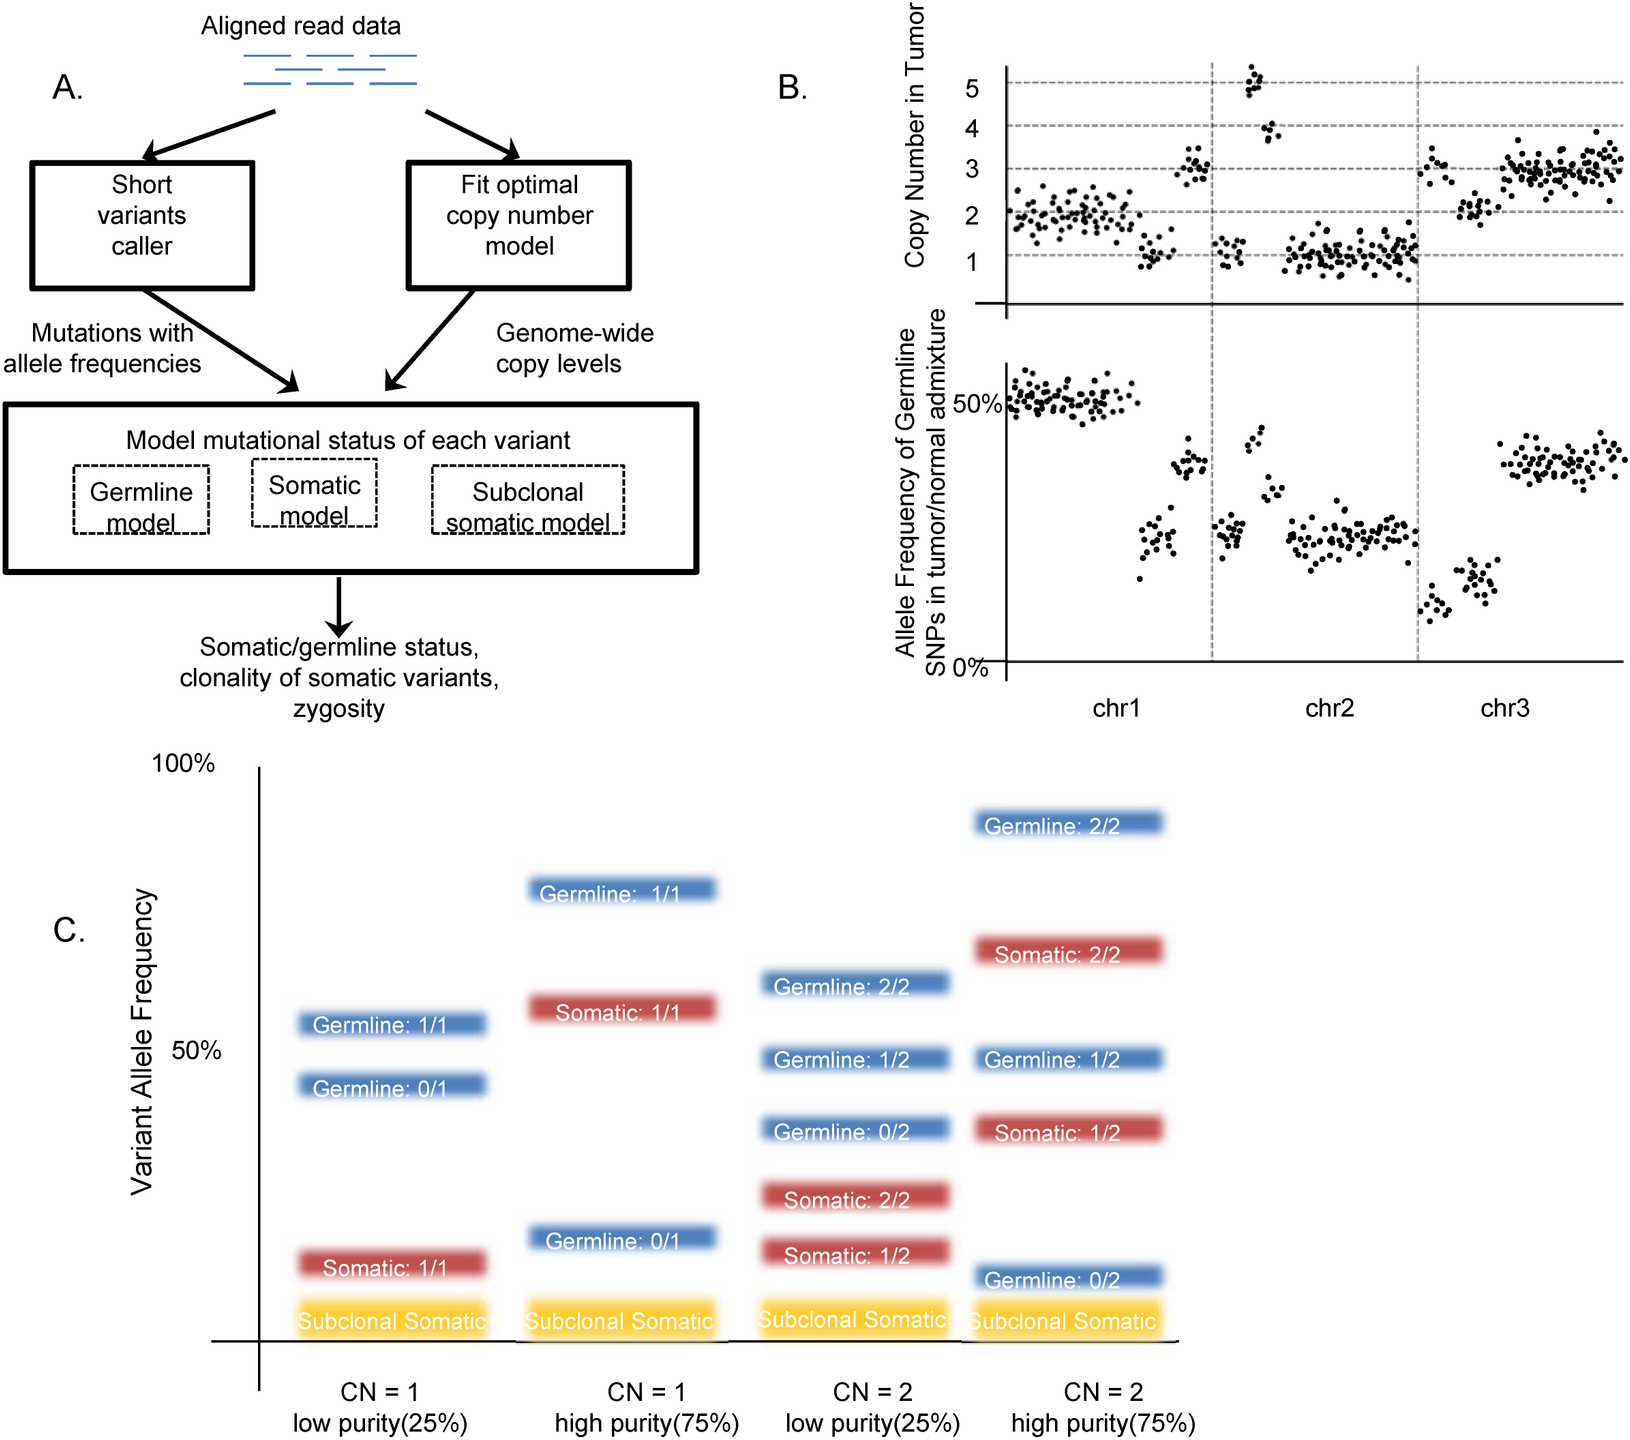
\includegraphics{journal.pcbi.1005965.g001.PNG}

\end{frame}

\begin{frame}{Allele frequency in Somatic vs Germline in tumor only
sample}
\protect\hypertarget{allele-frequency-in-somatic-vs-germline-in-tumor-only-sample}{}

\begin{itemize}
\tightlist
\item
  BRCA1 mutation: Positive - p.Glu649Ter (c.1945G\textgreater{}T)\\
\item
  Variant allele frequency 63.84\%\\
\item
  Tumor cell percentage: 70\%
\end{itemize}

\end{frame}

\begin{frame}{Allele frequency\textsuperscript{1}}
\protect\hypertarget{allele-frequency-sun_2018_computational_ploscomputationalbiology}{}

\(AF_{germline}\) \(=\) \({pV+1-p} \over {pC+2(1-p)}\) \(AF_{somatic}\)
\(=\) \(pV \over pC+2(1-p)\)

\begin{itemize}
\tightlist
\item
  Given copy number (C)
\item
  Variant allele count (V)
\item
  Sample purity (p)
\item
  Variant status (somatic or germline)
\end{itemize}

\end{frame}

\begin{frame}{Table of expected mutational allele
frequencies\textsuperscript{1}}
\protect\hypertarget{table-of-expected-mutational-allele-frequencies-sun_2018_computational_ploscomputationalbiology}{}

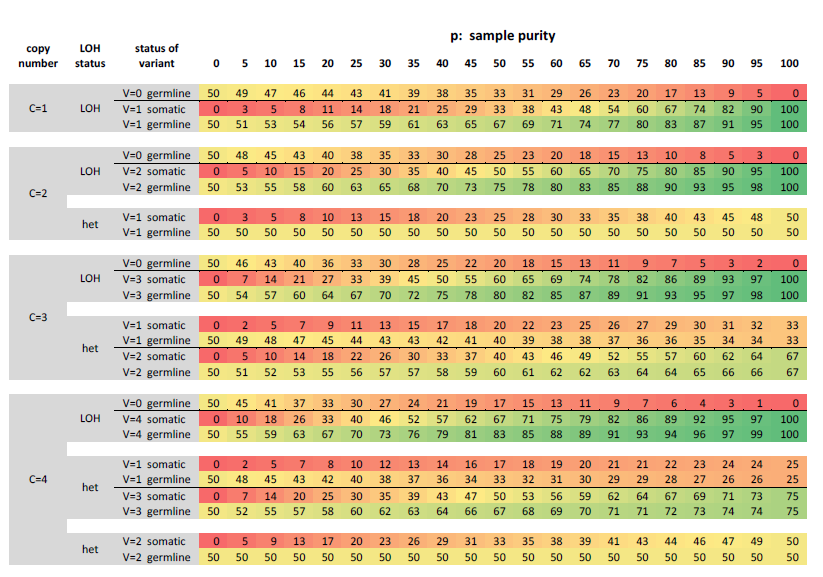
\includegraphics{AF.png}
\url{https://journals.plos.org/ploscompbiol/article/file?id=10.1371/journal.pcbi.1005965.s003\&type=supplementary}

\end{frame}

\begin{frame}{Limited information}
\protect\hypertarget{limited-information}{}

\begin{itemize}
\tightlist
\item
  What we know

  \begin{itemize}
  \tightlist
  \item
    Tumor cell percentage\\
  \item
    Variant allele frequency\\
  \end{itemize}
\item
  What we don`t know

  \begin{itemize}
  \tightlist
  \item
    Copy number\\
  \item
    LOH
  \end{itemize}
\end{itemize}

\end{frame}

\begin{frame}{Error}
\protect\hypertarget{error}{}

\begin{itemize}
\tightlist
\item
  Tumor cell percentage
\item
  Allele frequency
\end{itemize}

\[Allele \space frequency \not\approx Read \space count\]

\end{frame}

\begin{frame}{BRCA somatic mutation with LOH\textsuperscript{2}}
\protect\hypertarget{brca-somatic-mutation-with-loh--dejonge_2018_validation_thejournalofmoleculardiagnostics}{}

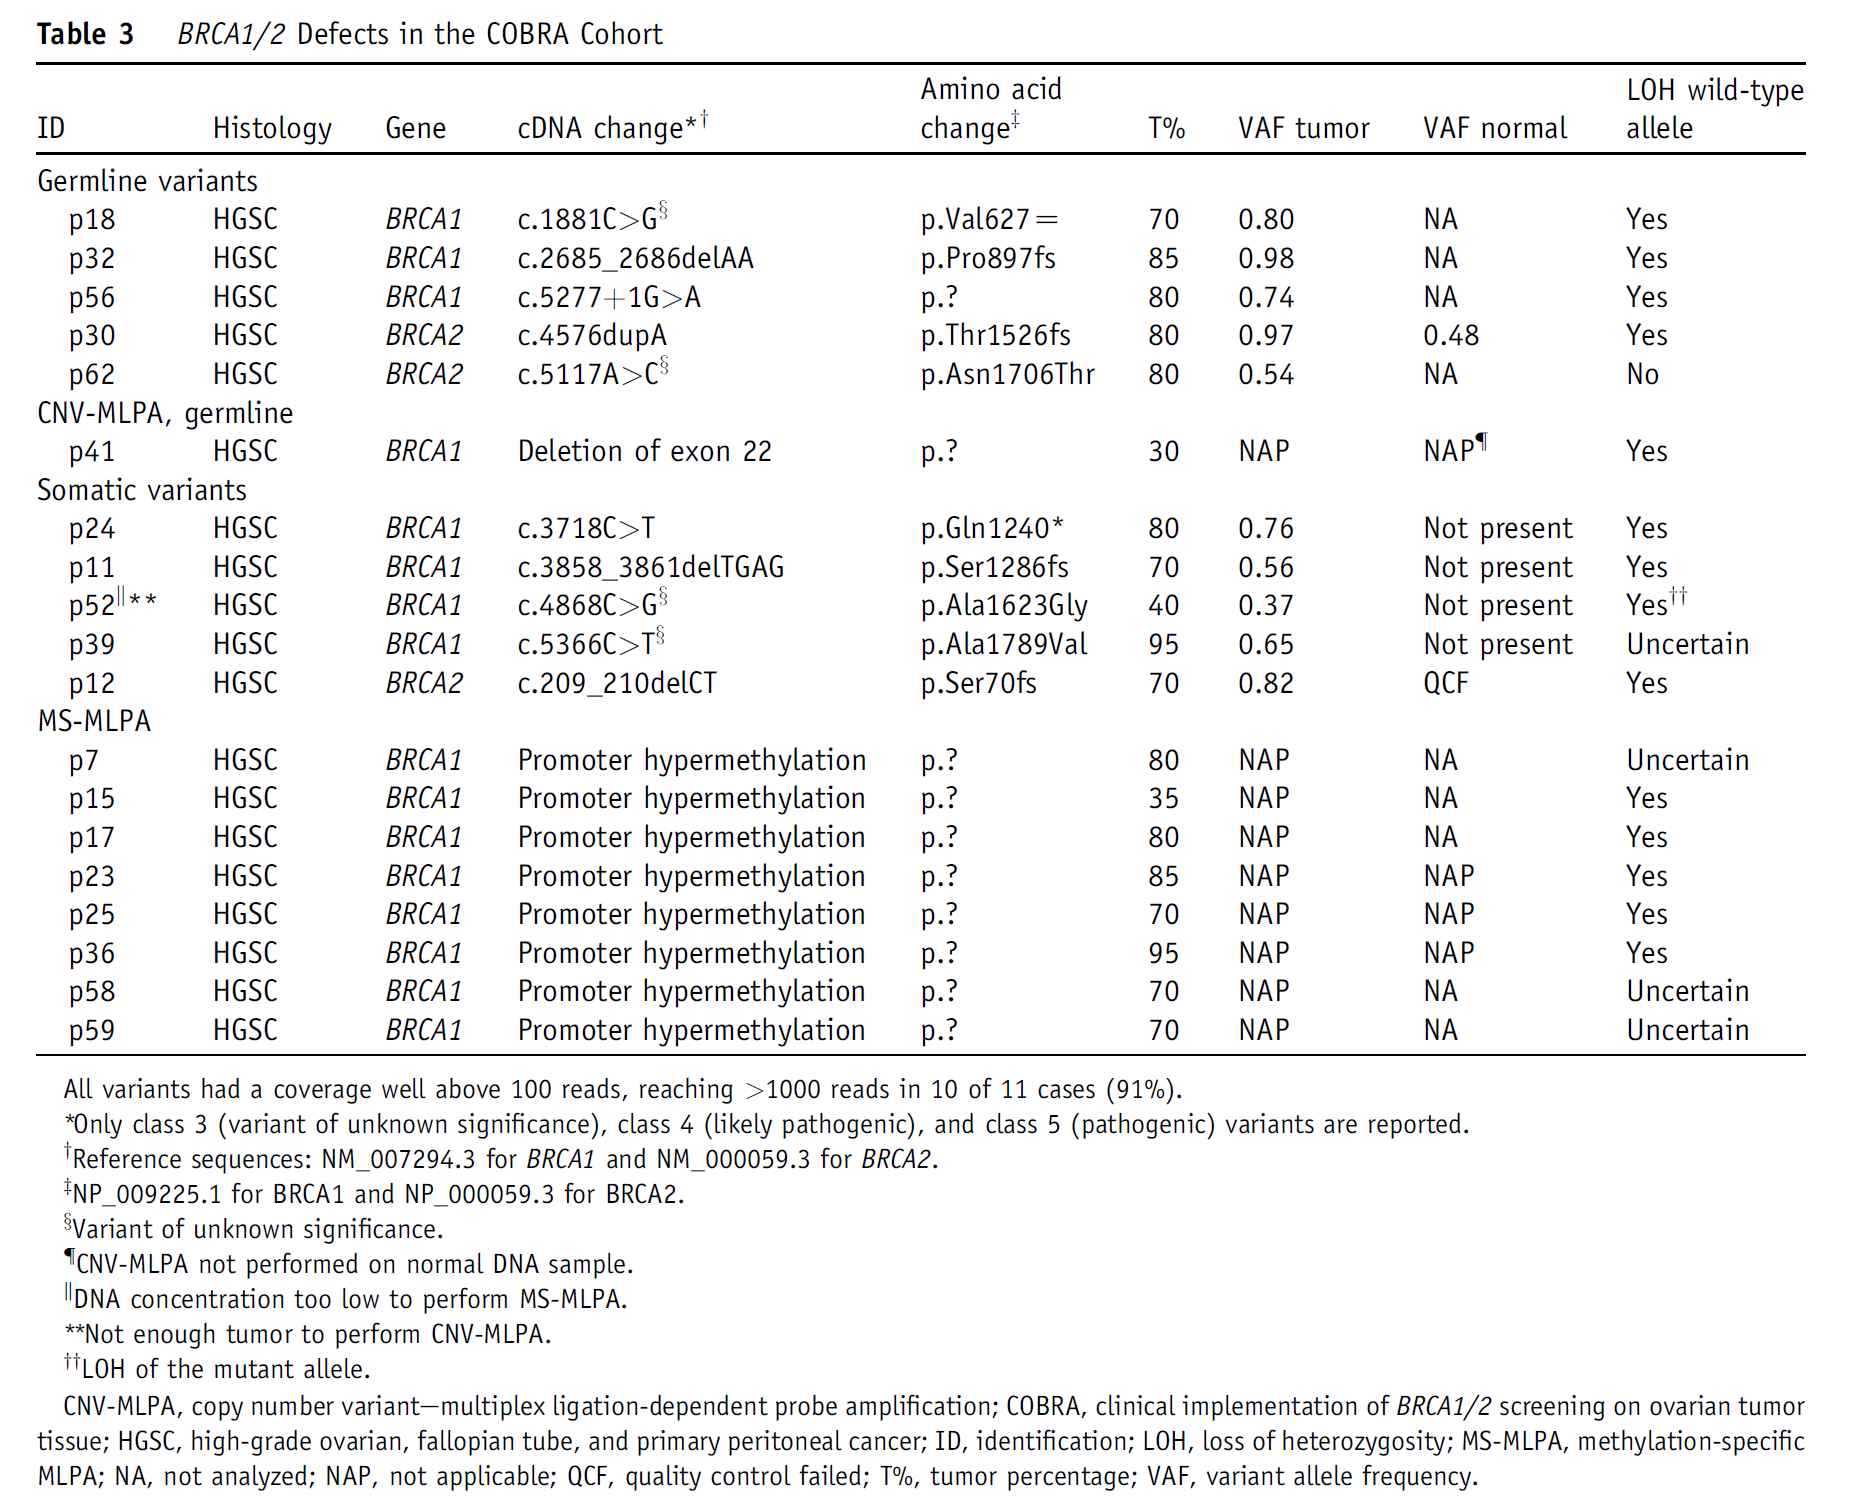
\includegraphics{LOH.png}

\end{frame}

\begin{frame}{Allele frequency in Somatic vs Germline in tumor only
sample}
\protect\hypertarget{allele-frequency-in-somatic-vs-germline-in-tumor-only-sample-1}{}

\begin{itemize}
\tightlist
\item
  BRCA1 mutation: Positive - p.Glu649Ter (c.1945G\textgreater{}T)\\
\item
  Variant allele frequency 63.84\%\\
\item
  Tumor cell percentage: 70\% -\textgreater{} 80\%
\end{itemize}

Suppose * LOH\\
* One copy

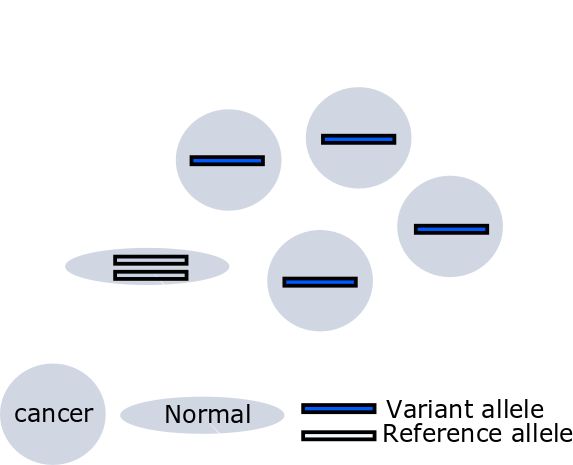
\includegraphics{img/Allele_12.png}

\(AF_{somatic}\) \(=\) \(pV \over pC+2(1-p)\) \(= 0.67\)

\end{frame}

\begin{frame}{Someone ask \ldots{}}
\protect\hypertarget{someone-ask}{}

\begin{quote}
Does tumor only NGS test distinguish a variant somatic and germline?\\
Answer `No'
\end{quote}

\begin{quote}
Is it possible \textbf{64\% allele frequency} of somatic BRCA variant?\\
Answer `Yes, It is when BRCA somatic variant accompanied with LOH'
\end{quote}

\end{frame}

\begin{frame}{References}
\protect\hypertarget{references}{}

\hypertarget{refs}{}
\leavevmode\hypertarget{ref-sun_2018_computational_ploscomputationalbiology}{}%
1. Sun, J.X., He, Y., Sanford, E., Montesion, M., Frampton, G.M.,
Vignot, S., Soria, J.-C., Ross, J.S., Miller, V.A., Stephens, P.J., et
al. (2018). A computational approach to distinguish somatic vs. Germline
origin of genomic alterations from deep sequencing of cancer specimens
without a matched normal. PLOS Computational Biology \emph{14},
e1005965.

\leavevmode\hypertarget{ref-dejonge_2018_validation_thejournalofmoleculardiagnostics}{}%
2. Jonge, M.M. de, Ruano, D., Eijk, R. van, Stoep, N. van der, Nielsen,
M., Wijnen, J.T., Haar, N.T. ter, Baalbergen, A., Bos, M.E.M.M., Kagie,
M.J., et al. (2018). Validation and Implementation of BRCA1/2 Variant
Screening in Ovarian Tumor Tissue. The Journal of Molecular Diagnostics
\emph{20}, 600--611.

\end{frame}

\end{document}
